
\section{Internet Video QoE}
\label{sec:measurement:video} 

\newcommand{\numsessions}{numsessions\xspace}
\newcommand{\problemsession}{problem session\xspace}
\newcommand{\problemsessions}{problem sessions\xspace}
\newcommand{\cluster}{cluster\xspace}
\newcommand{\clusters}{clusters\xspace}
\newcommand{\problemcluster}{problem cluster\xspace}
\newcommand{\problemclusters}{problem clusters\xspace}
\newcommand{\problemratio}{problem ratio\xspace}

\newcommand{\criticalcluster}{critical cluster\xspace}
\newcommand{\criticalclusters}{critical clusters\xspace}

In this section, we begin by describing our dataset and
metrics under consideration.
Then we present preliminary statistics on today's 
video QoE to motivate 
the types of structural insights we would
like to obtain regarding the nature of video 
quality problems. 

\subsection{Dataset and QoE Metrics}
\label{subsec:measurement:video:dataset}

Our dataset is based on client-side measurements of
video  quality from over 300 million sessions over a duration
of two weeks. The unique feature of our dataset is that it is 
collected over 379 distinct content providers spanning diverse 
genres, both live and video-on-demand content, different 
content delivery platforms, different types of  bitrate adaptation 
algorithms, and device/browser platforms. 
Though US viewers dominates the dataset ($\sim$55\%), 
there are a fair number of European ($\sim$12\%) and 
Chinese ($\sim$8\%) users in the dataset.
This is especially relevant as it provides us with a panoramic 
view   of state of  Internet video delivery today.

The basic unit in our dataset is a video session. 
A session represents a user viewing a video on one of 
our affiliates' sites for some duration of time.
Each session is associated with a set of \emph{seven 
features}: 
\begin{packedenumerate}
\item \emph{ASN:} The Autonomous System Number 
(ASN) that the client IP belongs  to. 
Note that a single ISP (e.g., Comcast) may own 
different ASNs both  for management and business reasons. 
We focus on the ASN as it is more fine-grained
than the ISP granularity.  We observe in aggregate 
15K unique ASNs spanning multiple countries. 

\item \emph{CDN:}   In total, we observe 19 unique CDNs 
spanning popular CDN providers as well as several in-house 
and ISP-run CDNs. (Some providers use proprietary 
CDN switching logic; in this case we pick the segment of 
the session with the CDN used for the longest
duration.)


\item \emph{Content provider (Site):} This is the specific 
provider from which the client requested some content. 
We have  379 content providers that span different 
genres of content.  We use the terms site and
content provide interchangeably.

\item \emph{VoD or Live:} Video  content  falls in one 
 of two categories: video-on-demand (VoD) or Live.  
 We use a binary indicator to see if the particular
  content was a Live event or a 
 VoD video. 


\item \emph{Player type:} We see diverse  players 
such as  Flash, Silverlight, and HTML5.

\item \emph{Browser:} We see diverse client browsers 
including Chrome, Firefox, MSIE, and Safari. 

\item \emph{Connection type:} Finally, we  have the 
type of access network connection such  as
 mobile/fixed wireless, DSL, fiber-to-home. 
These annotations come from third party services~\cite{quova}.
 
\end{packedenumerate}


We focus on  four key QoE metrics that are common across 
different  content providers and have been shown to be
 critical for measuring quality as well as user
  engagement~\cite{sigcomm11}: 
\begin{packedenumerate}
%\vyas{how is a join failure detected?}
\item \emph{Buffering ratio:}  Given a video session of 
duration $T$~seconds,  if the player spent $B$~seconds in 
buffering (i.e., waiting for the 
 buffer to replenish), the buffering ratio is defined as 
 $\frac{B}{T}$. 
 Prior work has shown that buffering ratio is a key metric
 that impacts user engagement~\cite{sigcomm11}.

\item \emph{Join time:}  This is the time taken for the video 
to start playing  from the time the user clicks on the ``play'' 
button. 
 While join time may not directly impact the view time of a 
 specific video,
 %the amount of a specific video viewed, 
 it does have long term effects as it reduces the likelihood 
 of repeated visits~\cite{sigcomm11,imc12akamai}.  
 

\item \emph{Average bitrate:} 
Many video players today support adaptive bitrate
selection and midstream bitrate switching to adapt to 
changing bandwidth availability. 
The average bitrate of a session is the time-weighted
average of the bitrates used in a given session. 
%(Bitrate refers to the video playback rate, rather than throughput or download rate.)


\item \emph{Join failures:}   Some sessions may not even 
start playing the video; either the content is not available
 on the CDN server or the CDN is under overload or other 
unknown reasons. We mark as a session as a join failure
if no content was played during this session.
%\footnote{Join failures are
%reported by the client-side measurement module that sends a ``heartbeat'' on
%the player status.}


\end{packedenumerate}


\begin{figure*}[th]
\centering
\captionsetup[subfigure]{justification=centering,farskip=-1pt,captionskip=5pt}
\subfloat[Buffering ratio]{
   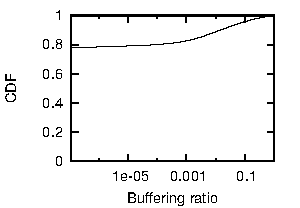
\includegraphics[width=0.32\textwidth] {figures/value_buffering.pdf}
 }
\subfloat[Bitrate]{
   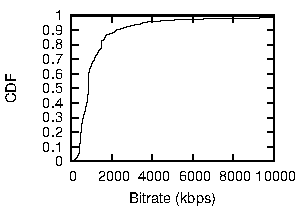
\includegraphics[width=0.32\textwidth] {figures/value_bitrate.pdf}
 }
\subfloat[Join time]{
   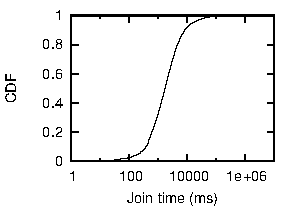
\includegraphics[width=0.32\textwidth] {figures/value_jointime.pdf}
 }
\caption{Distributions of observed QoE metrics -- 
buffering ratio, average bitrate, and join time. 
 We see that a non-trivial number of sessions suffer quality problems. 
 For instance, more than 5\% of sessions have a buffering ratio larger
  than 10\%.  }
\label{fig:overview:qualitycdf}
\end{figure*}


\subsection{How is the Video QoE today?}
\label{subsec:measurement:video:today}

Figure~\ref{fig:overview:qualitycdf} shows the distribution of the 
first three quality metrics over the 1-week dataset.  
(Join failures are binary events; it is not meaningful to look at a 
distribution.) 
The result reconfirms prior observations that there are a non-trivial 
number of sessions with less-than-ideal 
quality~\cite{sigcomm11,sigcomm12}. 
The key difference here is that  these past efforts only considered 
a small set of 3--4 content providers. 
In contrast,   we are considering the aggregate data from over 
300 content providers. 
For instance, more than 5\% of all sessions have a join time greater 
than 10~seconds; i.e., users had to wait for 10 seconds before the 
video even started playing! Similarly, more than 5\% of sessions 
had a buffering ratio that was greater than 10\%.  
This is particularly bad as past studies show that even a 1\% 
increase in buffering ratio can lead to 3-4 minutes of lost 
viewership~\cite{sigcomm11}.  
Finally, we also see that more than 80\% of sessions observe 
an average  bitrate less than 2~Mbps; 
i.e., less than the lower end of today's ``HD'' content.   
Note that the dataset from which I made these observations 
is dominated by  US-based content providers whose viewers 
have good broadband penetrations, and QoE could be worse in 
less developed regions.less than the lower end of 
today's ``HD'' content.   

\subsection{Methodology of Structural Analysis}
\label{subsec:measurement:video:method}

Now that we see that many video sessions suffer from bad QoE, 
we would like to know whether there is any patterns of these 
video quality problems.
In particular, we are interested in the temporal and spatial patterns 
of QoE problems:
\begin{itemize}
\item Temporally, is each problem a transient or one-off event for 
a specific ISP, CDN, or provider (or combination of these) or are 
these problems persistent over long periods?
\item Spatially, are the problems uniformly spread through the 
space of feature combinations or are there specific 
combinations that have a higher concentration?
\end{itemize}

\mypara{Identifying problem sessions} 
Our focus  is on understanding quality problems as they appear 
in the wild. 
To this end, we identify \problemsessions w.r.t. each of the 
quality metrics. Note that a given session may appear as a 
\problemsession on a subset of  metrics; i.e., it might have a low
join time but may have a high buffering ratio or vice versa. 
We consider the  metrics separately to avoid implicitly 
assuming that the metrics or failures are correlated.

\begin{packeditemize}
\item For join failures, we use a binary indicator if the 
session failed or not.  
For the remaining metrics, we choose specific 
thresholds based on domain-specific
knowledge and observations in prior work\footnote{
We do acknowledge that there is no ideal choice of 
threshold and it is likely that these thresholds will evolve 
as user expectations and network conditions improve. 
As such, the choice of thresholds is illustrative of the 
structure of video quality problems that occur today. 
The methodology and qualitative observations we 
present are not  tied to the  specific  thresholds.
We have confirmed that the results are qualitatively 
similar for other choices  of these thresholds as well. }.  
Our specific thresholds and rationale are follows.
\item For buffering ratio, we identify a \problemsession 
if the value is greater than 5\%; this is based on the 
observation that beyond this value there is a sharp 
decrease in amount of video viewed~\cite{sigcomm11}.  
\item For bitrate, we mark a \problemsession if the average
bitrate is less than 700kbps; this value roughly
 corresponds to the recommended ``360p'' setting on 
 video providers. 
We use a fixed threshold of bitrate in this work for 
simplicity, but we do acknowledge that bitrate settings 
are content-dependent (e.g., some contents do not provide 
high resolution streams).
\item Third,  we mark all sessions with a join
time greater than 10 seconds; this represents a 
conservative upper bound on the
tolerance of users~\cite{webhci1,akamai-imc12}.  
\end{packeditemize}

\mypara{Identifying problem clusters}
 We begin by dividing our dataset into discrete one 
 hour epochs.\footnote{One hour is the finest 
 granularity of the dataset and thus we cannot 
 analyze effects at smaller timescales.} As a
first step to analyze the structure, we 
\emph{cluster}\footnote{The term ``cluster'' represents a 
group of sessions that share common features, and it is 
indeed  different from traditional   clustering algorithms 
where a cluster can be a group of any data points.} 
together sessions that share one or more client/session 
features within the same epoch.   
For instance, the \cluster ``ASN=$\mathit{ASN1}$'' describes 
all sessions where the user belongs
to $\mathit{ASN1}$ and the cluster 
``ASN=$\mathit{ASN1}$, CDN=$\mathit{CDN1}$'', 
describes all sessions where the
user belongs to $\mathit{ASN1}$ and the session was 
assigned to a server from $\mathit{CDN1}$.
In order for our observations to be reliable, 
we want to focus on  clusters that are deemed to be 
statistically significant sources of problem sessions. 
To this end, we define the \problemratio of a
cluster as the ratio 
$\frac{\textrm{\# of \problemsessions}}{\textrm{\# of
sessions}}$. Then, we cull out the \clusters whose 
\problemratio is
significantly higher than the global average \problemratio.  
We also remove all \clusters that have a small number 
of sessions in aggregate; i.e., problems observed within a 
small cluster may not be statistically significant.
Combining these two steps, we define a \problemcluster 
as a \cluster that has a \problemratio $\geq 1.5 \times$ the
global \problemratio,\footnote{This value roughly represents 
two standard deviations away  from the mean of the
per-cluster \problemratio distribution.}  and the number of 
sessions in this cluster is $\geq1000$.  
In the rest of this paper, we start from the \problemclusters 
as our basis and subsequently refine the analysis.
 

\begin{figure*}[t]
\centering
\captionsetup[subfigure]{justification=centering,farskip=-1pt,captionskip=5pt}
\subfloat[Representing the relationship between clusters using a DAG.  
Red boxes represent the \problemclusters.
%The dashed-green boxes show clusters without a high \problemratio and the solid-red boxes identify the \problemclusters.
]{
   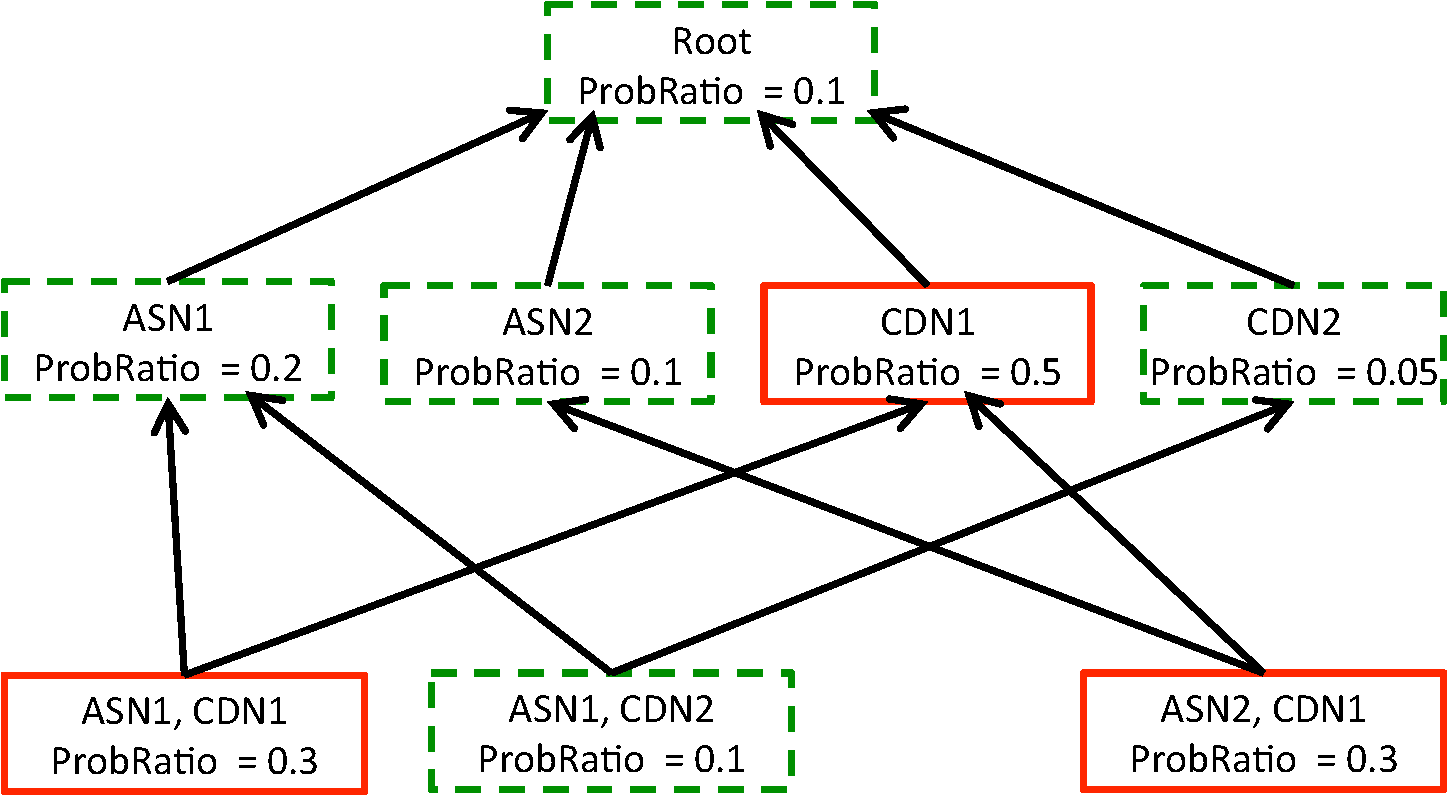
\includegraphics[width=0.47\textwidth] {figures/conext13-criticalcluster.pdf}
   \label{fig:method:critcluster}
 }
 \hspace{0.4cm}
\subfloat[An illustration of the phase transition idea for  identifying a \criticalcluster. 
%Intuitively,  removing any one feature from this \criticalcluster will cease to 
%be a \problemcluster and adding any feature  to it will continue to be a \problemcluster.
]{
   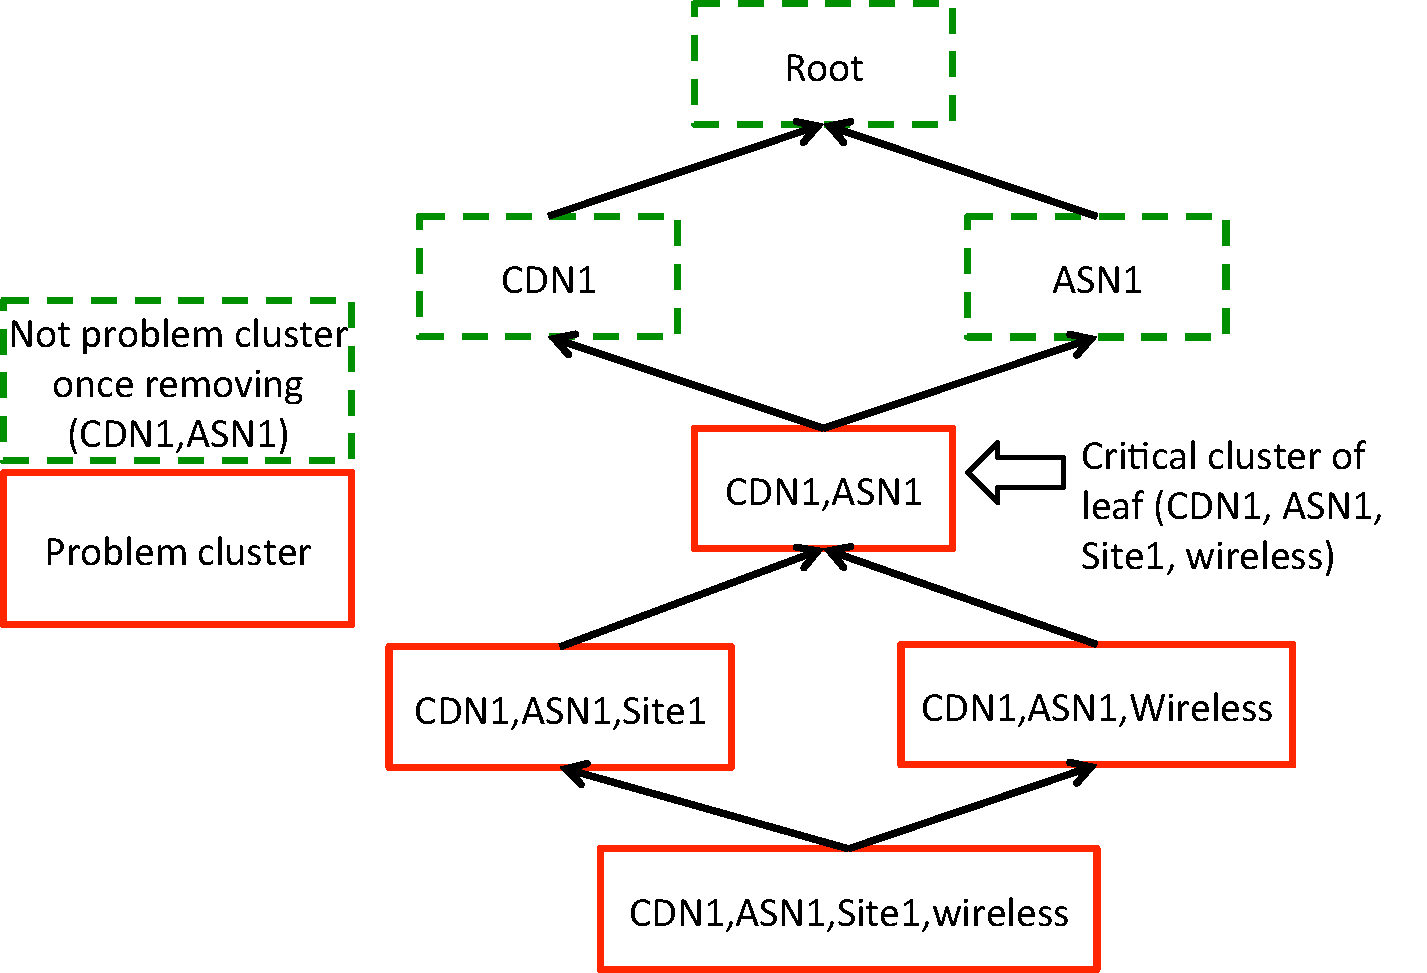
\includegraphics[width=0.47\textwidth] {figures/conext13-criticalcluster_example.pdf}
   \label{fig:method:critclustr2}
 }
\caption{Illustrative examples of how to identify \criticalclusters from \problemclusters.}
\label{fig:pattern:method}
\end{figure*}

While the grouping of problem sessions into \problemclusters  
provides some insights into the structure of problems, 
there is still one key missing aspect. 
Specifically, we may have different granularities of \problemclusters
that may be intrinsically related to the same underlying root cause.
Thus, our next step is to refine these \problemclusters to identify such
potential causal structures across the \problemsessions. 

The set of all \clusters can be viewed as a \emph{hierarchical}
structure across the space of client/session features 
 with natural parent-child relationships. We can visualize
these parent-child relationships as a DAG as shown in 
Figure~\ref{fig:method:critcluster}.  
A cluster $\mathit{C1}$ is a parent of cluster $\mathit{C2}$, 
if the set of features defining the  cluster $\mathit{C1}$
is a strict subset of that of $\mathit{C2}$. 
For instance, the  cluster ``$\mathit{ASN1}$'' is a parent of
the more specific clusters ``$\mathit{ASN1}$, $\mathit{CDN1}$'' 
and   `` $\mathit{ASN1}$, $\mathit{CDN2}$''. 


\mypara{Identifying critical clusters}
Our goal is to identify a small number of {\em \criticalclusters} 
that can potentially explain the occurrences of different 
\problemclusters.  
In our example in Figure~\ref{fig:method:critcluster}, intuitively 
we should pick the ``$\mathit{CDN1}$'' cluster rather than pick 
``$\mathit{ASN1}$, $\mathit{CDN1}$'' and ``$\mathit{ASN2}$, 
$\mathit{CDN2}$'' clusters separately.
Given that we do not have ground truth, \criticalclusters can 
serve as  starting points for further investigation. 
%
An intuitive criterion for  identifying a \criticalcluster is 
analogous to the notion of the minimum description length 
(or Occam's razor) from the machine learning literature. 
Conceptually, we should pick the most  compact description
to explain an observation.  Building on the above intuition, 
we can identify a \criticalcluster as consisting of the minimal 
set of features that when combined together can lead to 
significantly high problem ratio in its \cluster
(e.g., a \problemcluster) and removing even one feature
 from this set will reduce the problem ratio. 
To this end, we identify \criticalclusters using a \emph{phase
transition} algorithm as follows. 
For each session, we construct all logical paths in the DAG 
from the root to the leaf.  
Then, for each of these paths, we identify the point closest 
to the root along this path such that every cluster that is a 
descendant  is a \problemcluster and once removing it every 
cluster that is an ancestor is not a \problemcluster.
We use Figure~\ref{fig:method:critclustr2} to explain the intuition. 
In this figure, ``$\mathit{CDN1}$, $\mathit{ASN1}$'' is the 
\criticalcluster---every cluster that is a child of
this combination is a \problemcluster and if we remove the 
sessions in this combination, the parents ``$\mathit{CDN1}$'' 
and ``$\mathit{ASN1}$'' cease to be \problemclusters.
That is, this combination of features represents a key 
``transition point'' in this hierarchy between \problemclusters 
and non-problem clusters. 


\subsection{Temporal Patterns}
\label{subsec:measurement:video:temporal}

We begin by analyzing the temporal \emph{prevalence} and 
\emph{persistence} of the \problemclusters.

\mypara{Prevalence of \problemcluster} 
We define the \emph{prevalence} of a \problemcluster as the 
fraction of the total number of epochs in which this cluster 
appears as a \problemcluster.  
% Consider the example in Figure~\ref{fig:method:temporal} with a
%total of 6 epochs, the prevalence of the cluster ``$ASN1$, $CDN1$'' is
%$\frac{4}{6} = 0.67$ and similarly the prevalence of the cluster ``$CDN2$'' is
%$\frac{5}{6} = 0.83$.  
Figure~\ref{fig:measure:prevalence} shows the distribution of 
the prevalence of the \problemclusters for the different
quality metrics. We see a consistent pattern  across all quality 
metrics that around 10\% of the clusters have a prevalence 
greater than 8\% across all metrics. 
In other words, many of these \problemclusters are repeated 
observations that are recurrent problem events. 

\mypara{Prevalence of \problemcluster}
We define the \emph{persistence} of a \problemcluster in terms 
of the length of the consecutive occurrences of this cluster as a
\problemcluster.  
To this end, we coalesce consecutive occurrences of the cluster 
into a single logical event that lasts for multiple hours. 
For each \problemcluster, we  consider the distribution of the 
length of these ``streaks'' and report the median value.
%\emph{median}  and the \emph{maximum}  value. 
%For the timeseries in Figure~\ref{fig:method:temporal}, the ``$ASN1$,$CDN1$'' cluster
%has a median and maximum persistence of 2 while the ``$ASN2$'' cluster has a
%maximum persistence of 4. (In this simple series, the median and max coincide,
%but more generally they will not.)
Figure~\ref{subfig:measure:persistence-median} shows 
the distribution of the median persistence. 
For three of the metrics, more than 60\% of the \problemclusters 
have a median duration that last more than 2 hours.



\begin{figure*}[t]
\centering
\captionsetup[subfigure]{justification=centering,farskip=-1pt,captionskip=5pt}
\subfloat[Distribution of the prevalence of  \problemclusters]{
   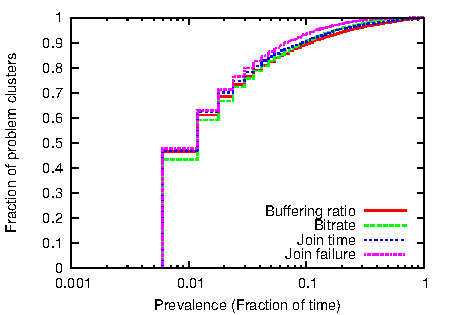
\includegraphics[width=0.45\textwidth] {figures/conext13-figure-cdf-sc-prevalence.pdf}
   \label{fig:measure:prevalence}
 }
\subfloat[Inverse CDF of the median persistence of \problemclusters]{
   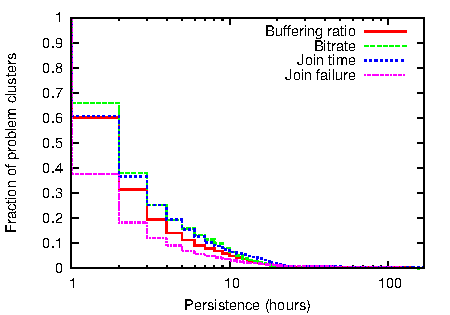
\includegraphics[width=0.45\textwidth] {figures/conext13-figure-cdf-sc-persistence-median.pdf}
   \label{subfig:measure:persistence-median}
 }
\caption{Distributions of the prevalence and persistence of  \problemclusters.
We find a natural skewed distribution with a few 
 clusters having high prevalence. 
 Many \problemclusters last multiple hours and that a non-trivial 
 number of \problemclusters last for tens of hours.}
\label{fig:}
\end{figure*}

\subsection{Spatial Patterns}
\label{subsec:measurement:video:spatial}

The previous results showed that there are a non-trivial 
number of persistent/prevalent \problemclusters that last for
several hours. 
As we discussed earlier,  multiple \problemclusters may 
be implicitly related by a single root cause as we saw in
Figure~\ref{fig:method:critcluster}.  
To this end, we focus next on the \criticalclusters using the 
algorithm described in 
Section~\ref{subsec:measurement:video:method}. 
Recall that every  \criticalclusters is also a \problemcluster; 
i.e.,  it has a sufficiently high problem ratio and it has a 
significant number of sessions. The motivation to focus on 
a few critical cluster rather than all \problemclusters is the 
observation (as shown shortly) that a small fraction of 
\problemclusters cover most of the \problemsessions.

\begin{figure}[t]
\centering
   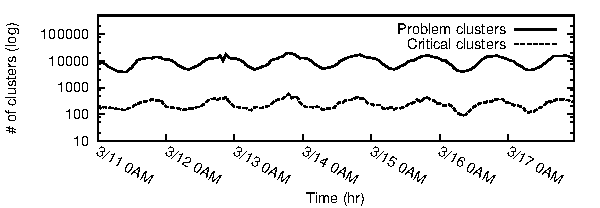
\includegraphics[width=0.7\textwidth] {figures/conext13-time-cluster-count-join-time.pdf}
%\vspace{-0.3cm}
\caption{The number of \criticalclusters is significantly  
smaller than the number of \problemclusters. 
The timeseries shown here  is for the join time; we see 
similar  results for the other quality metrics too.}
\label{fig:critical:reduction}
\end{figure}


\mypara{Critical cluster analysis}
Figure~\ref{fig:critical:reduction} shows the number of 
\problemclusters relative to the number of \criticalclusters 
in the case of the Join Time metric. 
We see that  number of \criticalclusters is almost 
50$\times$ lower than the number of \problemclusters 
suggesting that there are indeed a small number of 
events that might have ``caused''  most  problems.  
One natural question is whether  the \criticalclusters 
\emph{cover} most of the \problemsessions. 
Table~\ref{tab:critical:reduction} summarizes the mean 
coverage and reduction  of the \criticalclusters for the four 
quality metrics and in all cases, we see that the number of 
\criticalclusters is only   2-3\% of the number of 
\problemclusters (i.e., 50$\times$ fewer), but they manage to
cover 44--84\% of the \problemsessions. 
As a point of reference,  we also show the coverage of 
the \problemclusters; i.e., not  all sessions are part of a 
\problemcluster as they may be part of  small clusters or 
clusters with very small \problemratio. 
We see that the \criticalclusters cover almost all 
\problemsessions that are part of some \problemcluster; 
i.e., many of the coverage  gaps are really due to 
\problemsessions that belong to a statistically insignificant 
cluster (i.e., either with too few sessions or with 
too few \problemsessions).
 
 
\begin{table}[t]
\begin{center}
\begin{small}
\begin{tabular}{c|p{2cm}|p{2cm}|p{2.5cm}|p{2.5cm}}
Metric	& Mean \problemclusters & Mean \criticalclusters & Mean \problemcluster coverage & Mean \criticalcluster coverage\\ \hline 
BufRatio	 & 10433 & 286 (2\%) & 0.8 & 0.66 (82\%) \\
JoinTime & 9953 & 247 (2\%) & 0.86 & 0.83 (96\%) \\
JoinFailure & 9620 & 302 (3\%) & 0.87 & 0.84 (96\%)\\
Bitrate & 9437 & 287 (3\%) & 0.57 & 0.44 (77\%)
\end{tabular}
\end{small}
\end{center}
\caption{Reduction via focusing only on \criticalclusters 
and the effective coverage  of the \criticalclusters.}
\label{tab:critical:reduction}
\end{table}


Next, we analyze the structure of the \criticalclusters for 
the different quality metrics. 
First, we analyze the types of  client/session  feature 
combinations that appear frequently in the \criticalclusters. 
Then, we analyze if the different metrics are correlated in the 
\criticalclusters. Finally, we highlight some interesting 
observations  and some hypothesis to explain  
the most prevalent \criticalclusters. 



%\begin{figure}[t]
%\centering
%\captionsetup[subfigure]{justification=centering,farskip=-1pt,captionskip=5pt}
%\subfloat[BufferingRatio]{\label{subfig:measure:pie-bufferingratio}
%   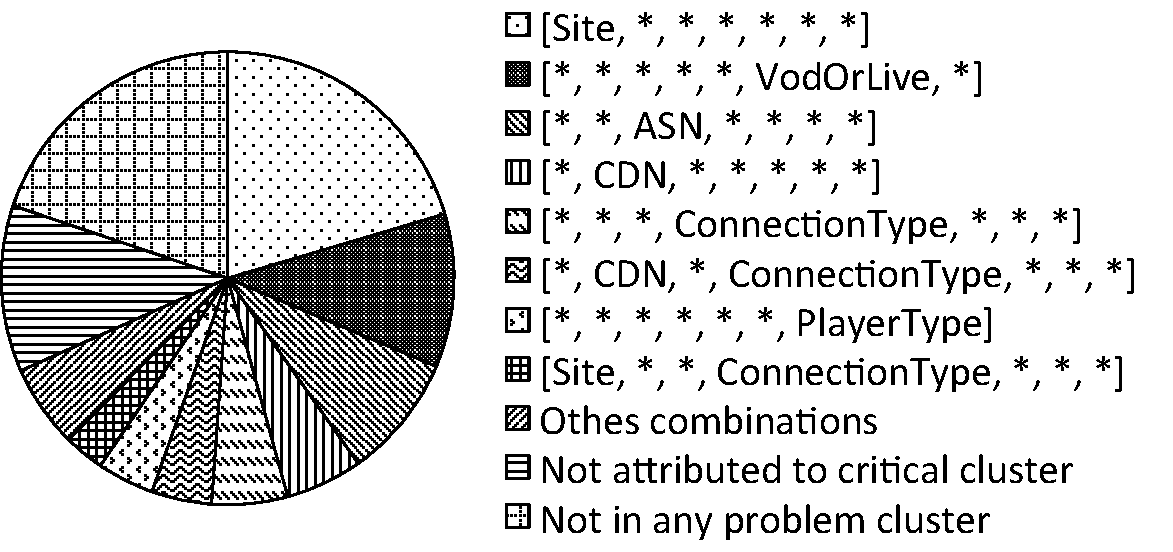
\includegraphics[width=0.48\textwidth] {figures/conext13-figure-pie-bufferingratio.pdf}
% }
%\subfloat[Bitrate]{\label{subfig:measure:pie-bitrate}
%   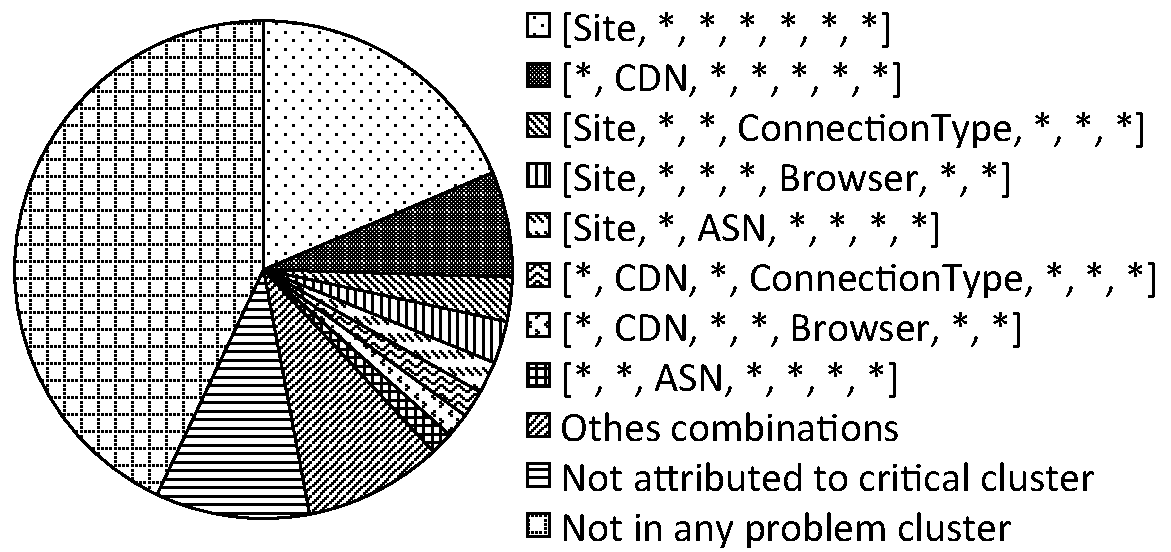
\includegraphics[width=0.48\textwidth] {figures/conext13-figure-pie-bitrate.pdf}
% }\\
%\subfloat[JoinTime]{\label{subfig:measure:pie-jointime}
%   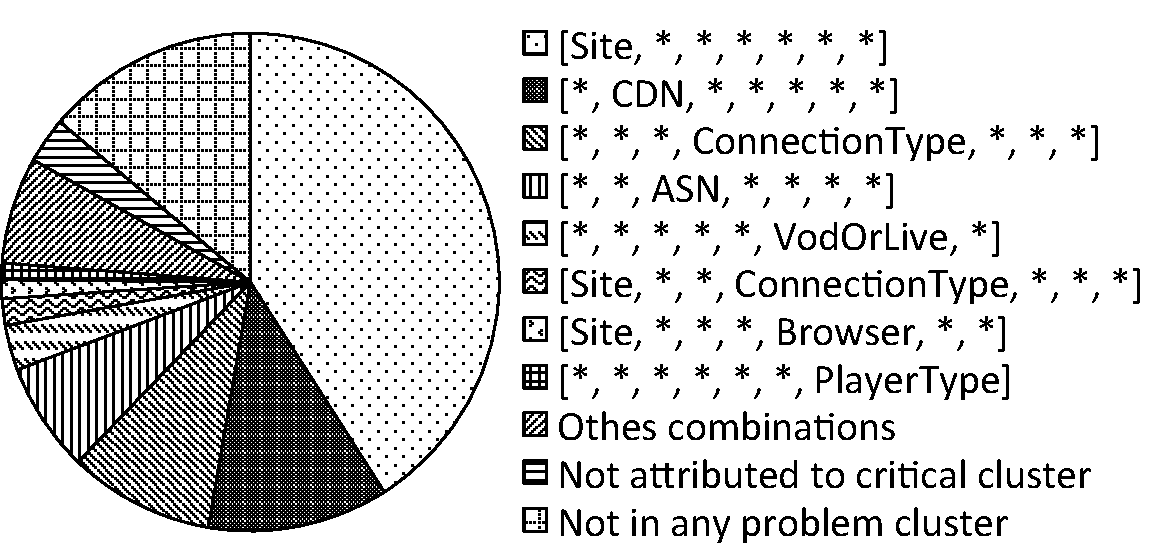
\includegraphics[width=0.48\textwidth] {figures/conext13-figure-pie-jointime.pdf}
% }
%\subfloat[JoinFailure]{\label{subfig:measure:pie-joinfailure}
%   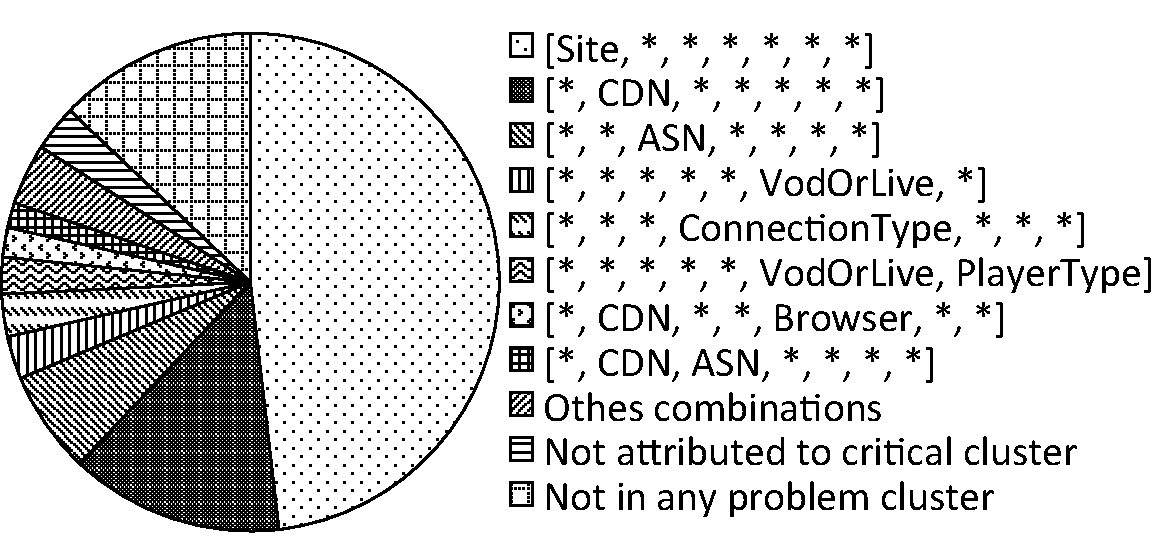
\includegraphics[width=0.48\textwidth] {figures/conext13-figure-pie-joinfailure.pdf}
% }
%\caption{Analyzing the structure of the \criticalclusters.
%The result show a breakdown of the total number of 
%sessions attributed to a specific type of \criticalcluster. 
%Note that there may be multiple values of these features;
%i.e., there can be many Sites and many CDNs  contributing 
%to the Site and CDN sector.}
%\label{fig:critical:pie}
%\end{figure}
%
%\mypara{Types of clusters} 
%Figure~\ref{fig:critical:pie} shows a breakdown of the 
%types of \criticalclusters  for different quality metrics.  
%We aggregate \criticalclusters into the different feature 
%dimension(s) they represent. 
%For instance, if we see a \criticalcluster for $CDN1$ and 
%$CDN2$, we count these toward the CDN contribution 
%in the pie chart.   
%Some \problemsessions may remain unaccounted for 
%in this breakdown for two reasons:
%(a) they are not part of a significant enough 
%\problemcluster or 
%(b) our algorithm did not assign a \criticalcluster for a 
%\problemcluster. 
%This mirrors   the coverage observation we saw earlier in 
%Figure~\ref{fig:critical:reduction}
% and  Table~\ref{tab:critical:reduction}. 
%In almost all cases, most of the unaccounted for sessions 
%fall outside any \problemcluster;  i.e., this is not due to 
%the \criticalcluster detection algorithm. 
%The result shows that the most dominant category of 
%\criticalclusters actually corresponds to a
%\emph{content provider} (labeled as ``Site'').  
%We also see that CDN, ASN, and ConnectionType are
% also prominent types of \criticalclusters across all 
% quality metrics. 
%This suggests that most quality issues are potentially 
%caused by server-side (Site or CDN) or client-side 
%(ASN, ConnectionType) problems rather than a 
%combination (which indicates a bad path between 
%client and server) or other features.

%This is
%related to the coverage observation we saw earlier---with the exception of the
%bitrate category, the coverage is quite high.
 
%Note that this does not mean that the same set of \criticalclusters appear
%across all metrics as we will see next.


\mypara{Understanding most prevalent  \criticalclusters} 
In order to illustrate the causes for the problem,  we 
consider the \criticalclusters with a prevalence higher 
than 60\% for the different quality metrics. 
For clarity of presentation, we only consider the 
\criticalclusters whose features fall in one of the following 
categories: ASN, CDN, Site, and ConnectionType as
our previous breakdown shows these as the most 
dominant features.  
We present this analysis with two disclaimers.  
First, due to the sensitive nature of this data, we do not 
present the names of the actual providers, but focus on their
characteristics.  
Second, this involves a fair amount of manual analysis and
domain knowledge. As such, we intend this result to be 
illustrative (and somewhat speculative) rather than attempt 
to be conclusive.  
This said, we still believe that the high-level insights are 
still useful to inform future video delivery architectures.

Table~\ref{tab:depth} presents some of the anecdotal 
examples we observed.  
The empty cells simply indicate that there were no 
\criticalclusters in this category with a prevalence higher 
than 60\%. 
We see a few interesting patterns here.  
In terms of buffering ratio, we see that the top ASNs are 
typically in Asia, and the content providers that had issues 
typically only had a single bitrate of content. 
The CDNs with buffering/join time problems are also
typically ``in-house'' CDNs run by the Site itself; i.e., 
not a third-party CDN like Akamai or Limelight.  
We also see that wireless connections and wireless
ISPs appear in the buffering and bitrate cells 
respectively, which is somewhat expected. 


One interesting artifact we uncovered in the case of 
join time was that these were mostly ASNs in China 
accessing content from Chinese CDNs but there were
third-party player modules loaded from US providers 
that led to higher join times. Another curious 
observation is that all the Sites with significant join
failures tended to use the same global CDN. 
However, the CDN in aggregate does not have a 
significant presence in terms of failures, except in the 
case of these Sites.\footnote{These Sites used a single 
CDN; recall that our \criticalcluster algorithm will 
prefer more compact descriptions and thus
features these problems to the Site rather than the 
single Site-CDN combination.} 
We speculate that these, presumably low-end, 
providers may have lower priority service and could 
have potentially benefited from using multiple CDNs.


\begin{table}[t]
\begin{center}
\begin{small}
\begin{tabular}{p{1.5cm}|p{3.5cm}|p{2.5cm}|p{3.5cm}|p{2.5cm}}
		& ASN &  CDN   & Site  & ConnType  \\ \hline 

BufRatio	 & Asian ISPs  & In-house, single bitrate   & Single bitrate &  Mobile wireless  \\   \hline
JoinTime 	&  Chinese ISPs accessing CDNs in China, but player loads modules from US CDN	& In-house CDNs of UGC providers & High bitrates  \\  \hline 
JoinFailure 	&   & Same set as buffering ratio & Same single global CDN, maybe low priority providers &  \\ \hline 
Bitrate 	& Wireless provider &   & UGC Sites &    
\end{tabular}
\end{small}
\end{center}
\caption{Analysis of the most  prevalent \criticalclusters. 
A empty cell implies that we found no interesting 
 cluster in this combination.}
\label{tab:depth}
\end{table}


\mypara{Overlap across metrics} 
%We saw in the previous  graph that the types of
% \criticalclusters that contribute the most 
% \problemsessions are very similar across different 
%quality metrics.  
%Note, however, that this does not necessarily mean 
%that the actual set of \criticalclusters are identical. 
%In other words, a different set of CDNs or Sites may 
%be responsible for problems across buffering ratio and
%join time. 
Next, we would like to know how much the \criticalclusters
of different quality metrics correlate with each other.
In other words, a different set of CDNs or Sites may 
be responsible for problems across buffering ratio and
join time. 
To analyze this, we compute the \emph{Jaccard similarity} 
index between the top-100 in terms of the total number 
of \problemsessions covered  \criticalclusters  
for the different metrics. 
(The Jaccard similarity measure for two sets A and B 
is $\frac{|A \cap B|}{|A \cup B|}$.)
We find that the overlap between the different 
metrics is only around 23\% in the best case (buffering 
ratio and join time) and in the worst case is only around
1\% (between bitrate and join failure).  
We manually analyzed the specific clusters and we 
found that  the actual set of Site, CDN, and ASN
\criticalclusters are indeed very different.  

%We look at this in more depth next.
 


%\begin{table}[t]
%\begin{center}
%\begin{small}
%\begin{tabular}{c|c|c|c|c}
%		& Buffering Ratio & Join Time & Join failure & Bitrate \\ \hline 
%Buffering Ratio	 & \fillme & 0.22 & 0.13 & 0.07 \\
%Join Time & \fillme & \fillme & 0.09 & 0.08 \\
%Join failure & \fillme & \fillme & \fillme & 0.008 \\
%Bitrate & \fillme & \fillme & \fillme & \fillme 
%\end{tabular}
%\end{small}
%\end{center}
%\tightcaption{Average Jaccard similarity index between the top-\fillme \criticalclusters for the different metrics. 
% We see that most metrics are relatively uncorrelated, possibly because the 
% critical features are very different.}
%\end{table}

\begin{table}[t]
\begin{center}
\begin{small}
\begin{tabular}{p{2cm}|p{2cm}|p{2cm}|p{2cm}|p{2cm}|p{2cm}}
	BufRatio vs. Bitrate & BufRatio vs. JoinTime & BufRatio vs. JoinFailure & Bitrate vs. JoinTime & Bitrate vs. JoinFailure & JoinTime vs. JoinFailure\\ \hline 
0.07 & 0.23 & 0.13 & 0.08 & 0.01 & 0.09 \\
\end{tabular}
\end{small}
\end{center}
\caption{Average Jaccard similarity index between the top 
100 \criticalclusters for the different metrics. 
 We see that most metrics are relatively uncorrelated, possibly because the 
 critical features are very different.}
\end{table}




\subsection{Key Observations}
\label{subsec:measurement:video:findings}

Our key observations from the analysis of \problemclusters 
and  \criticalclusters  are:  

\begin{packeditemize}

\item There is a distinct skewed distribution  in the prevalence; 
around 8-12\% of the \problemclusters appear more than 
10\% of the time.

\item There is also a skewed distribution  in the persistence; 
more than 20\% of  \problemclusters have a median duration 
greater than 2 hours.  

\item We find that a small number of \criticalclusters 
(2-3\% of the number of \problemclusters) can account 
for 44-84\% of all \problemsessions. 

\item While the set of feature combinations in the 
\criticalclusters that cover the most number of 
\problemsessions is very similar across the quality
metrics (i.e., Site, CDN, ASN), the actual values of 
these features is very different (with a max overlap of 23\%). 

\item  We see a few expected patterns  such as Asian 
and wireless ISPs appearing  as most prevalent \criticalclusters. 
We  see some unexpected patterns that can be easily alleviated 
(e.g., the player modules loaded remotely for Chinese users) 
and Sites that could benefit from standard strategies such as 
using more fine-grained bitrates or using multiple CDNs.

\end{packeditemize}



